\documentclass[../Kamil_Kowalewski_Main.tex]{subfiles}

\begin{document} {

    Niniejszy rozdział zawiera pełną dokumentację użytkownika aplikacji. Jego celem
    jest omówienie wszystkich dostępnych funkcji z~punktu widzenia osoby korzystającej
    z~aplikacji.

    \section{Wprowadzenie do obsługi interfejsu aplikacji}
    \label{chapter5:dok_uzytkownika:wprowadzenie_interface}{
        Interfejs aplikacji w~swoim zamyśle był tworzony zgodnie z~zasadami ergonomii,
        prostoty oraz intuicyjnej obsługi. Na rysunku
        \ref{chapter5:dok_uzytkownika:wprowadzenie_interface:ui_intro}
        został przedstawiony ekran powitalny aplikacji, warto dodać, że jest
        on wyświetlany gdy użytkownik nie jest zalogowany.
        \begin{figure}[H]
            \centering
            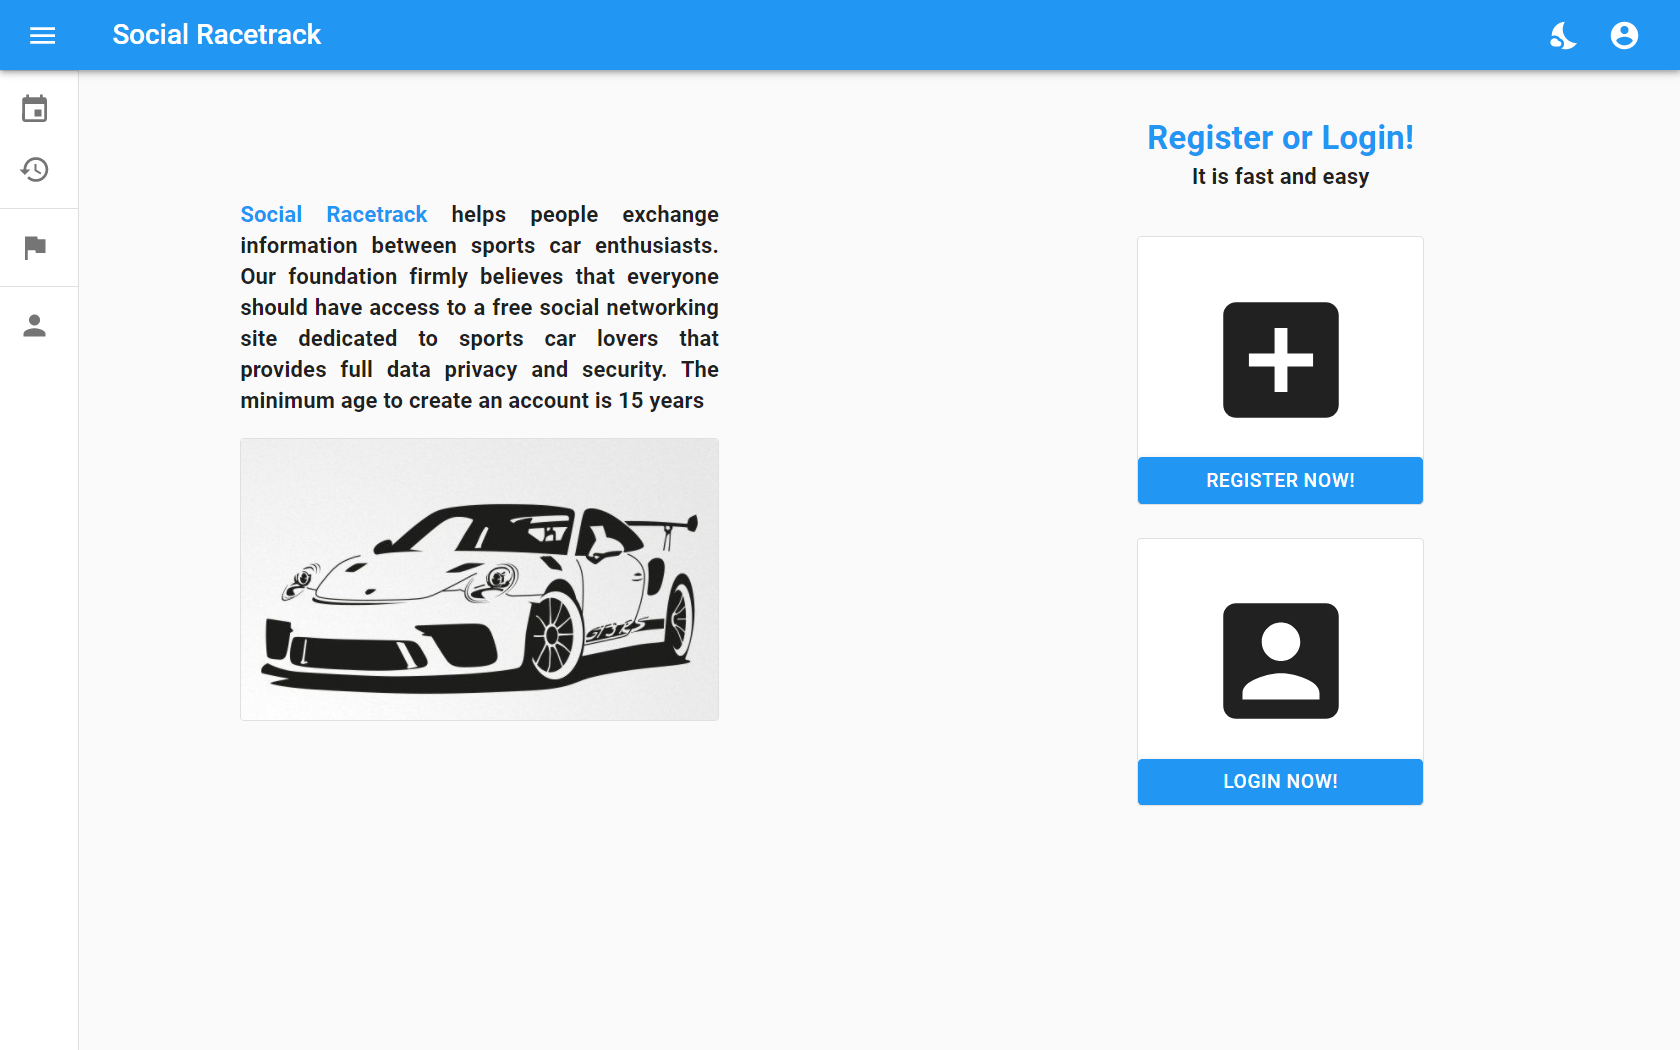
\includegraphics[width=0.7\textwidth, keepaspectratio]
            {img/chapter5/intro/UI_intro.png}
            \caption
            [Ekran powitalny aplikacji]
            {Ekran powitalny aplikacji}
            \label{chapter5:dok_uzytkownika:wprowadzenie_interface:ui_intro}
        \end{figure}

        Posiada on opcję zmiany barw aplikacji, dostępne opcje to jasna i~ciemna.
        Pierwsza z~nich została przedstawiona na rysunku
        \ref{chapter5:dok_uzytkownika:wprowadzenie_interface:ui_intro}. Aby dokonać
        zmiany należy nacisnąć przycisk w~prawym górnym rogu. Na rysunkach
        \ref{chapter5:dok_uzytkownika:wprowadzenie_interface:dark_mode} oraz
        \ref{chapter5:dok_uzytkownika:wprowadzenie_interface:light_mode}
        zostały przedstawione dwie różne ikony zależnie w~jakim trybie znajduje
        się aplikacja.
        \begin{figure}[H]
            \centering
            \begin{minipage}[b]{0.45\textwidth}
                \centering
                
\includegraphics[width=0.22\textwidth, keepaspectratio]
                {img/chapter5/intro/to_dark_mode.png}
                \caption
                [Przycisk do przełączania do trybu ciemnego]
                {Przycisk do przełączania do trybu ciemnego}
                \label{chapter5:dok_uzytkownika:wprowadzenie_interface:dark_mode}
            \end{minipage}
            \hfill
            \begin{minipage}[b]{0.45\textwidth}
                \centering
                
\includegraphics[width=0.22\textwidth, keepaspectratio]
                {img/chapter5/intro/to_light_mode.png}
                \caption
                [Przycisk do przełączania do trybu jasnego]
                {Przycisk do przełączania do trybu jasnego}
                \label{chapter5:dok_uzytkownika:wprowadzenie_interface:light_mode}
            \end{minipage}
        \end{figure}

        W~celu otwarcia bocznego panelu znajdującego się po lewej stronie należy nacisnąć
        przycisk przedstawiony na rysunku
        \ref{chapter5:dok_uzytkownika:wprowadzenie_interface:sidebar_open_button}.
        \begin{figure}[H]
            \centering
            
\includegraphics[width=0.1\textwidth, keepaspectratio]
            {img/chapter5/intro/open_sidebar.png}
            \caption
            [Przycisk do otwierania bocznego panelu]
            {Przycisk do otwierania bocznego panelu}
            \label{chapter5:dok_uzytkownika:wprowadzenie_interface:sidebar_open_button}
        \end{figure}

        Akcja ta zapewnia otwarcie bocznego panelu i~wyświetlenie opisu poszczególnych
        przycisków. Przycisk \textit{Future Events} odpowiada za wyświetlanie wydarzeń,
        które odbędą się w przyszłości. Przycisk \textit{Past Events} ma za zadanie
        wyświetlanie wydarzeń, które już się odbyły. Kolejny przycisk
        \textit{Racetracks} dokonuje prezentacji dostępnych obiektów sportowych.
        Ostatni dostępny przycisk \textit{Members} zapewnia możliwość
        przedstawienia użytkowników aplikacji. W celu schowania bocznego paska należy
        nacisnąć przycisk przedstawiony na rysunku
        \ref{chapter5:dok_uzytkownika:wprowadzenie_interface:sidebar_close_button}.
        \begin{figure}[H]
            \centering
            \begin{minipage}[b]{0.4\textwidth}
                \centering
                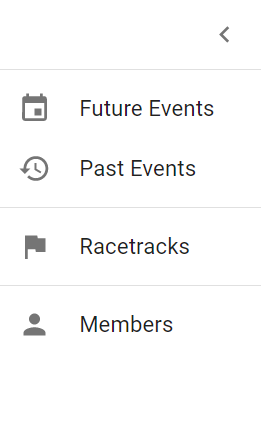
\includegraphics[width=0.6\textwidth, keepaspectratio]
                {img/chapter5/intro/sidebar.png}
                \caption
                [Boczny panel]
                {Boczny panel}
                \label{chapter5:dok_uzytkownika:wprowadzenie_interface:sidebar}
            \end{minipage}
            \hfill
            \begin{minipage}[b]{0.4\textwidth}
                \centering
                
\includegraphics[width=0.2\textwidth, keepaspectratio]
                {img/chapter5/intro/close_sidebar.png}
                \caption
                [Przycisk do zamykania bocznego panelu]
                {Przycisk do zamykania bocznego panelu}
                \label{chapter5:dok_uzytkownika:wprowadzenie_interface:sidebar_close_button}
            \end{minipage}
        \end{figure}

        W~celu logowanie lub rejestacji użytkownika należy skorzystać z przedstawionych
        na rysunkach
        \ref{chapter5:dok_uzytkownika:wprowadzenie_interface:register_button} oraz
        \ref{chapter5:dok_uzytkownika:wprowadzenie_interface:login_button}
        przycisków.
        \begin{figure}[H]
            \centering
            \begin{minipage}[b]{0.4\textwidth}
                \centering
                
\includegraphics[width=0.4\textwidth, keepaspectratio]
                {img/chapter5/intro/register_button.png}
                \caption
                [Przycisk do rejestracji użytkownika]
                {Przycisk do rejestracji użytkownika}
                \label{chapter5:dok_uzytkownika:wprowadzenie_interface:register_button}
            \end{minipage}
            \hfill
            \begin{minipage}[b]{0.4\textwidth}
                \centering
                
\includegraphics[width=0.4\textwidth, keepaspectratio]
                {img/chapter5/intro/login_button.png}
                \caption
                [Przycisk do logowania użytkownika]
                {Przycisk do logowania użytkownika}
                \label{chapter5:dok_uzytkownika:wprowadzenie_interface:login_button}
            \end{minipage}
        \end{figure}

        Inną możliwością jest skorzystania z~przycisku konta użytkownika,
        przedstawionego na rysunku
        \ref{chapter5:dok_uzytkownika:wprowadzenie_interface:account_button},
        który przenosi do okna logowania analogicznie jak przycisk przedstawiony na
        rysunku \ref{chapter5:dok_uzytkownika:wprowadzenie_interface:login_button}.
        \begin{figure}[H]
            \centering
            
\includegraphics[width=0.1\textwidth, keepaspectratio]
            {img/chapter5/intro/account_button.png}
            \caption
            [Przycisk konta użytkownika]
            {Przycisk konta użytkownika}
            \label{chapter5:dok_uzytkownika:wprowadzenie_interface:account_button}
        \end{figure}
    }

    \section{Obsługa aplikacji dla użytkownika niezalogowanego}
    \label{chapter5:dok_uzytkownika:obsluga_niezalogowany} {
        Zgodnie z~wymaganiami funkcjonalnymi i~niefunkcjonalnymi określonymi w~sekcji
        \ref{chapter4:dok_techniczna:wymagania} akcje dostępne dla użytkownika
        niezalogowanego są mocno ograniczone. Dla takiego użytkownika dostępny jest
        ekran powitalny przedstawiony na rysunku
        \ref{chapter5:dok_uzytkownika:wprowadzenie_interface:ui_intro} oraz możliwość
        wyświetlania obiektów sportowych oraz szczegółów na ich temat. Na rysunkach
        \ref{chapter5:dok_uzytkownika:obsluga_niezalogowany:racetracks} oraz
        \ref{chapter5:dok_uzytkownika:obsluga_niezalogowany:racetrack_details}
        zostały przedstawione strony wyświetlające wszystkie obiekty
        sportowe oraz szczegóły na temat tego, który został wybrany przez użytkownika.
        Aby wyświetlić szczegóły danego obiektu sportowego należy nacisnąć myszą
        na wybraną kartę z torem. W celu powrotu do ekranu przedstawionego na rysunku
        \ref{chapter5:dok_uzytkownika:obsluga_niezalogowany:racetracks} należy
        skorzystać z~przycisku powrotu w~przeglądarce.
        \begin{figure}[H]
            \centering
            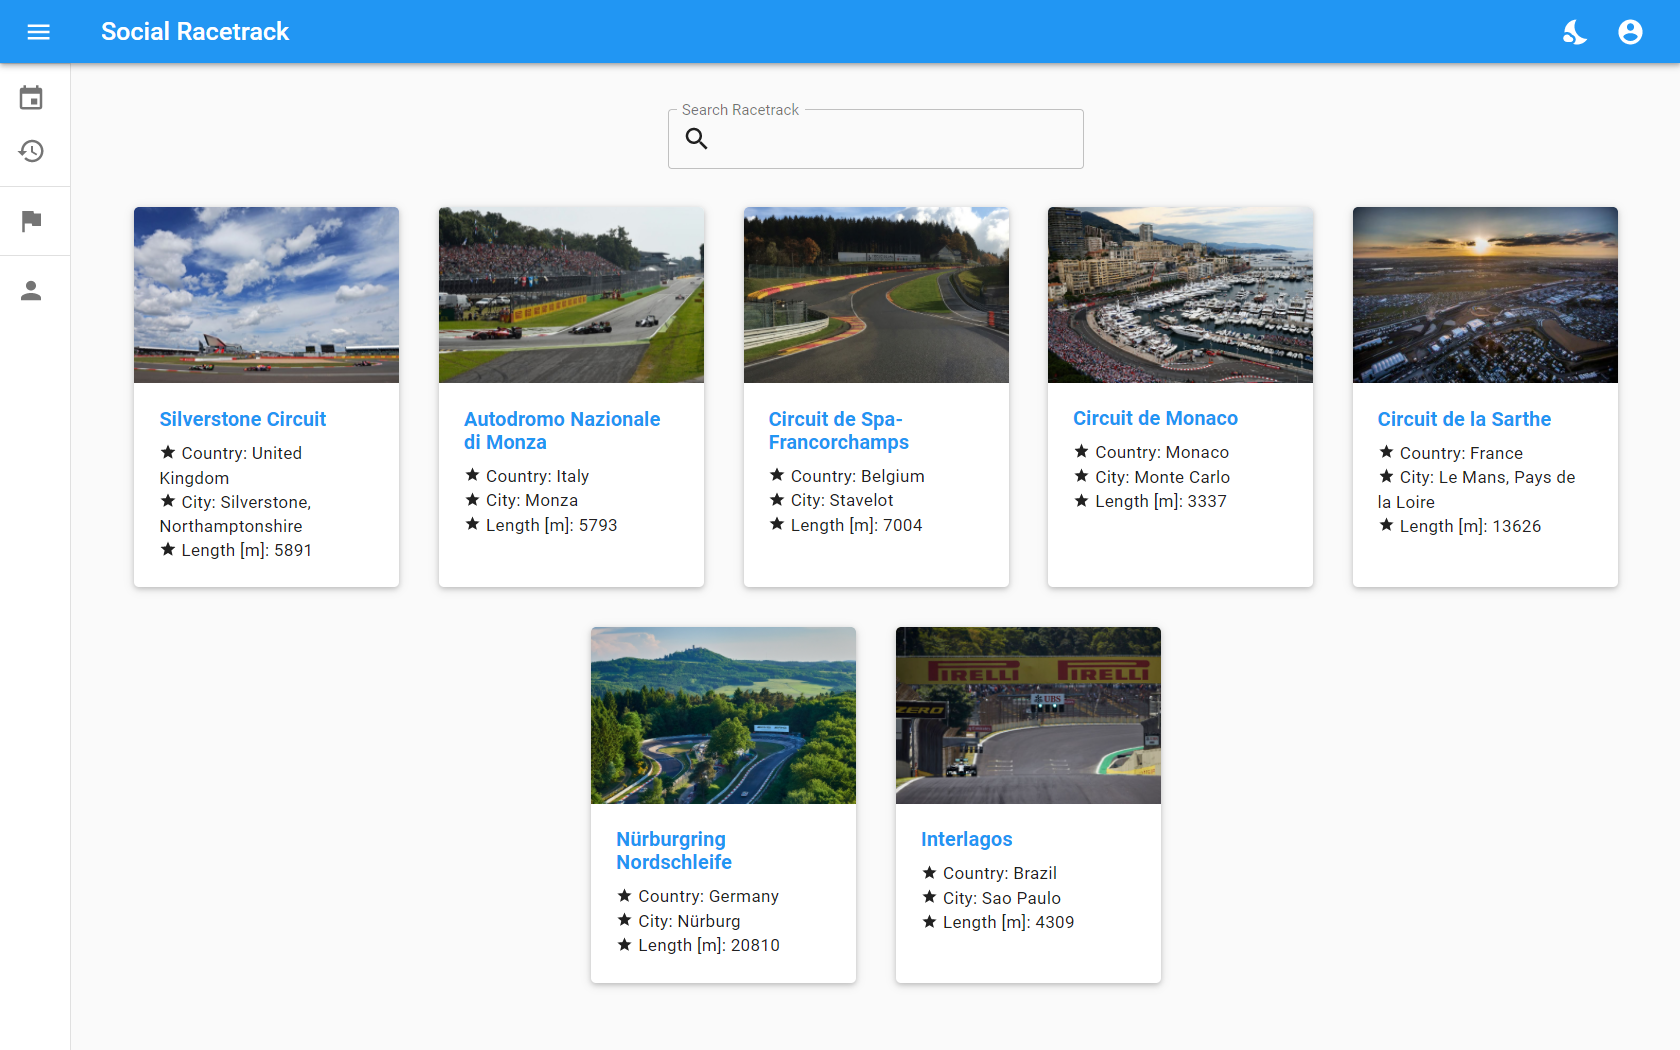
\includegraphics[width=0.7\textwidth, keepaspectratio]
            {img/chapter5/notloggedin/racetracks.png}
            \caption
            [Panel wyświetlający wszystkie obiekty sportowe]
            {Panel wyświetlający wszystkie obiekty sportowe}
            \label{chapter5:dok_uzytkownika:obsluga_niezalogowany:racetracks}
        \end{figure}

        \begin{figure}[H]
            \centering
            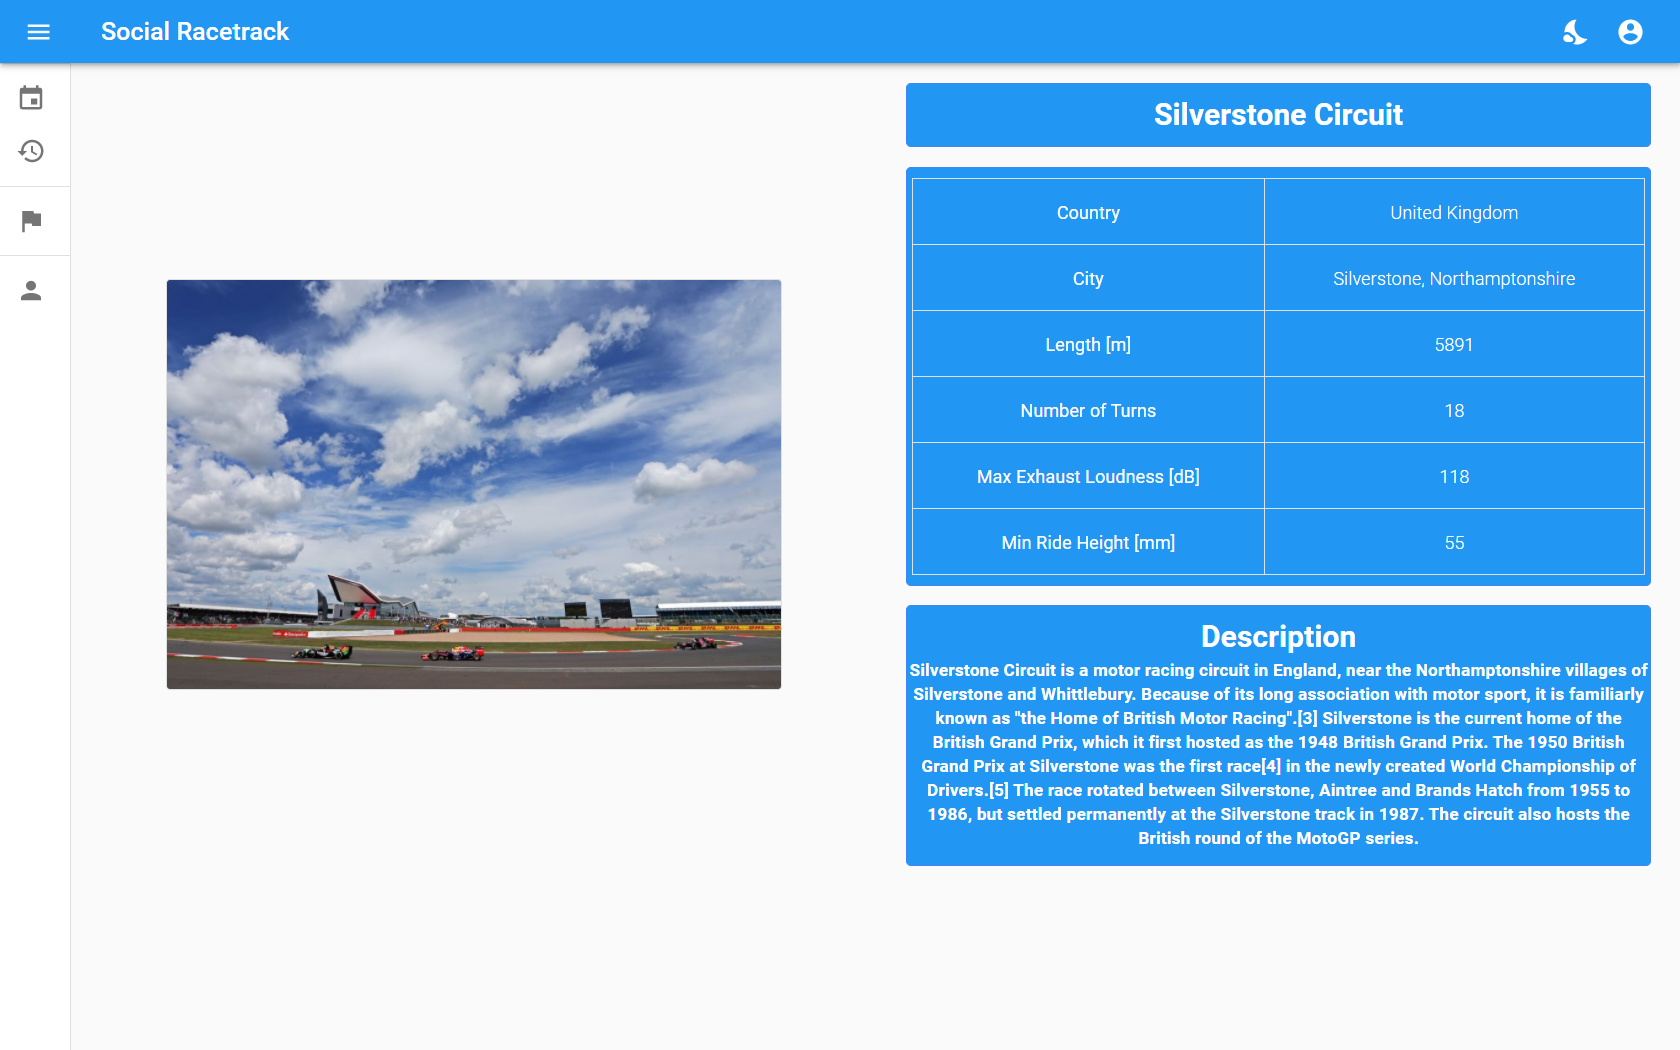
\includegraphics[width=0.7\textwidth, keepaspectratio]
            {img/chapter5/notloggedin/racetrack_details.png}
            \caption
            [Panel wyświetlający szczegóły na temat wybranego obiektu sportowego]
            {Panel wyświetlający szczegóły na temat wybranego obiektu sportowego}
            \label{chapter5:dok_uzytkownika:obsluga_niezalogowany:racetrack_details}
        \end{figure}
    }

    \section{Logowanie i rejestracja}
    \label{chapter5:dok_uzytkownika:logowanie_rejestracja} {
        Logowanie lub rejestracji odbywa się na specjalnie wydzielonej podstronie, aby
        uzyskać do niej dostęp należy skorzystać z~przycisków przedstawionych na
        rysunkach \ref{chapter5:dok_uzytkownika:wprowadzenie_interface:register_button},
        \ref{chapter5:dok_uzytkownika:wprowadzenie_interface:login_button} lub
        \ref{chapter5:dok_uzytkownika:wprowadzenie_interface:account_button}. Opis ich
        użycia został przedstawiony w~sekcji
        \ref{chapter5:dok_uzytkownika:wprowadzenie_interface}.

        Po wybraniu przycisku do rejestracji użytkownika zostanie wyświetlony panel
        przedstawiony na rysunku
        \ref{chapter5:dok_uzytkownika:logowanie_rejestracja:register_panel}.
        Należy go wypełnić zgodnie z~opisem każdego z~pól w formularzu a~następnie
        nacisnąć przycisk \textit{SIGN UP}. Po wykonaniu tej akcji zostanie
        przeprowadzone automatyczne zalogowanie na nowo utworzone konto
        a~następnie użytkownik zostanie poinformowany o~konieczności wylogowania. Po
        zakończeniu tych operacji użytkownik może się zalogować do swojego konta
        i~korzystać z~jego wszystkich funkcjonalności. W~przypadku posiadania już konta
        w~aplikacji i~otwarciu okna rejestracji możliwe jest przejście do panelu
        logowania poprzez naciśnięcie przycisku
        \textit{Already have an account? Sign in}.
        \begin{figure}[H]
            \centering
            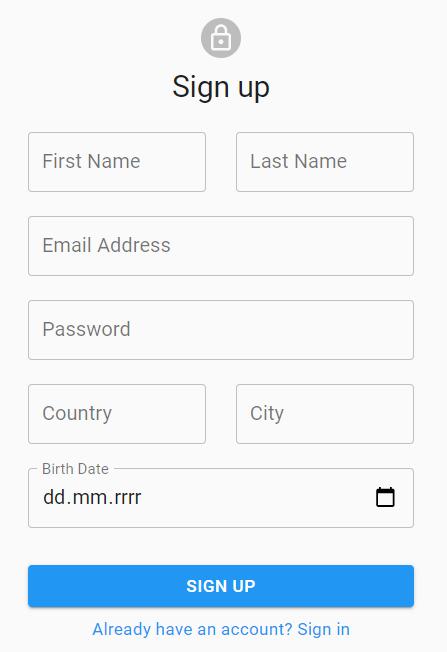
\includegraphics[width=0.35\textwidth, keepaspectratio]
            {img/chapter5/loginregister/register_panel.png}
            \caption
            [Panel rejestracji użytkownika]
            {Panel rejestracji użytkownika}
            \label{chapter5:dok_uzytkownika:logowanie_rejestracja:register_panel}
        \end{figure}

        Po wybraniu przycisku do logowania lub przycisku konta użytkownika zostanie
        wyświetlony panel przedstawiony na rysunku
        \ref{chapter5:dok_uzytkownika:logowanie_rejestracja:login_panel}.
        Należy go wypełnić zgodnie z~opisem każdego z~pól w~formularzu a~następnie
        nacisnąć przycisk \textit{SIGN IN}. Po tej akcji aplikacja wyświetli panel
        konta użytkownika. W przypadku nie posiadania konta w~aplikacji i~otwarcia okna
        logowania możliwe jest przejście do panelu rejestracji użytkownika poprzez
        naciśniecie przycisku \textit{Don't have an account? Sign Up}.

        W panelu logowania istnieje możliwość przywracania hasła, w~tym celu należy
        nacisnąć przycisk \textit{Forgot password?}. Po tej akcji zostanie otwarty
        panel przywracania hasła przedstawiony na rysunku
        \ref{chapter5:dok_uzytkownika:logowanie_rejestracja:reset_password},
        należy go wypełnić zgodnie z~opisem przedstawionym w~formularzu i~nacisnąć
        przycisk \textit{SEND EMAIL}. Na wskazany adres email zostanie wysłany link do
        zmiany hasła, należy go otworzyć i~postępować zgodnie ze wskazówkami w~nim
        przedstawionymi.
        \begin{figure}[H]
            \centering
            \begin{minipage}[b]{0.45\textwidth}
                \centering
                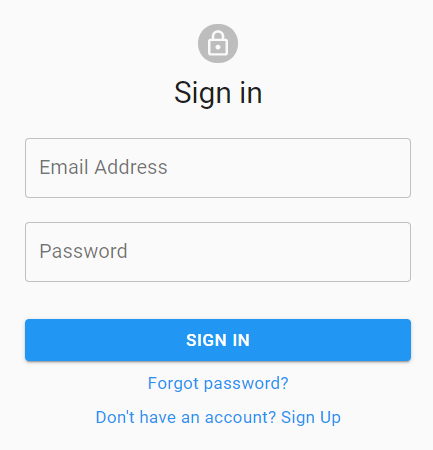
\includegraphics[width=0.7\textwidth, keepaspectratio]
                {img/chapter5/loginregister/login_panel.png}
                \caption
                [Panel logowania użytkownika]
                {Panel logowania użytkownika}
                \label{chapter5:dok_uzytkownika:logowanie_rejestracja:login_panel}
            \end{minipage}
            \hfill
            \begin{minipage}[b]{0.45\textwidth}
                \centering
                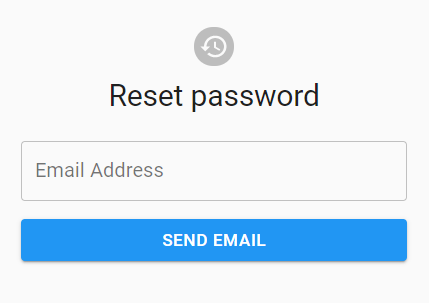
\includegraphics[width=0.7\textwidth, keepaspectratio]
                {img/chapter5/loginregister/reset_password.png}
                \caption
                [Panel przywracania hasła]
                {Panel przywracania hasła}
                \label{chapter5:dok_uzytkownika:logowanie_rejestracja:reset_password}
            \end{minipage}
        \end{figure}
    }

    \section{Obsługa funkcjonalności dostępnych dla użytkownika zalogowanego}
    \label{chapter5:dok_uzytkownika:funkc_uzyt_zalog} {

        \subsection{Obsługa konta użytkownika}
        \label{chapter5:dok_uzytkownika:funkc_uzyt_zalog:konto_uzyt} {
            Aby mieć możliwość dostępu do strony przedstawionej na rysunku
            \ref{chapter5:dok_uzytkownika:funkc_uzyt_zalog:user_panel} należy być
            zalogowanym i~należy nacisnąć przycisk pokazany na rysunku
            \ref{chapter5:dok_uzytkownika:wprowadzenie_interface:account_button}. Po
            wykonaniu tej akcji zostanie załadowany panel użytkownika. Składa się on
            z~kilku części ułożonych w~postaci poziomych pasów.

            Pierwszy z~nich zawiera awatar z~inicjałami użytkownika, obok niego jest
            przycisk, przedstawiony na rysunku
            \ref{chapter5:dok_uzytkownika:funkc_uzyt_zalog:add_button}, służący do
            dodawania pojazdów i~osiągnięć oraz edycji danych osobowych. Funkcjonalności
            te zostały opisane w~sekcjach
            \ref{chapter5:dok_uzytkownika:funkc_uzyt_zalog:konto_uzyt:dod_usun_samochod},
            \ref{chapter5:dok_uzytkownika:funkc_uzyt_zalog:konto_uzyt:dod_usun_nagrody} oraz
            \ref{chapter5:dok_uzytkownika:funkc_uzyt_zalog:konto_uzyt:edycja_danych},
            aby uzyskać do nich dostęp należy nacisnąć przycisk pokazany na rysunku
            \ref{chapter5:dok_uzytkownika:funkc_uzyt_zalog:add_button}.

            Drugi z~poziomych pasów zawiera dane osobowe użytkownika takie jak kraj, data urodzenia
            czy też email. Trzeci z~kolei przedstawia flotę pojazdów danego użytkownika
            oraz zapewnia opcje usuwania pojazdu, szczegółowo zostało to opisane w~sekcji
            \ref{chapter5:dok_uzytkownika:funkc_uzyt_zalog:konto_uzyt:dod_usun_samochod}.

            Trzeci z~poziomych pasów przedstawia listę zdobytych nagród przez
            użytkownika, analogicznie jak w~przypadku elementu wyświetlającego flotę
            pojazdów zapewniony jest przycisk do usuwania, które szczegółowo został
            opisany w~sekcji
            \ref{chapter5:dok_uzytkownika:funkc_uzyt_zalog:konto_uzyt:dod_usun_nagrody}.

            Ostatni poziomy pas, nie przedstawiony na rysunku
            \ref{chapter5:dok_uzytkownika:funkc_uzyt_zalog:user_panel} jest fragmentem
            odpowiedzialnym za wyświetlanie wydarzeń, w których brał lub będzie brał
            udział dany użytkownik. Wyświetlane są karty z~wydarzeniami analogicznie
            jak w~panelu przyszłych wydarzeń przedstawionym na rysunku
            \ref{chapter5:dok_uzytkownika:funkc_uzyt_zalog:przeglad_wydarz:future_events_panel}.

            \begin{figure}[H]
                \centering
                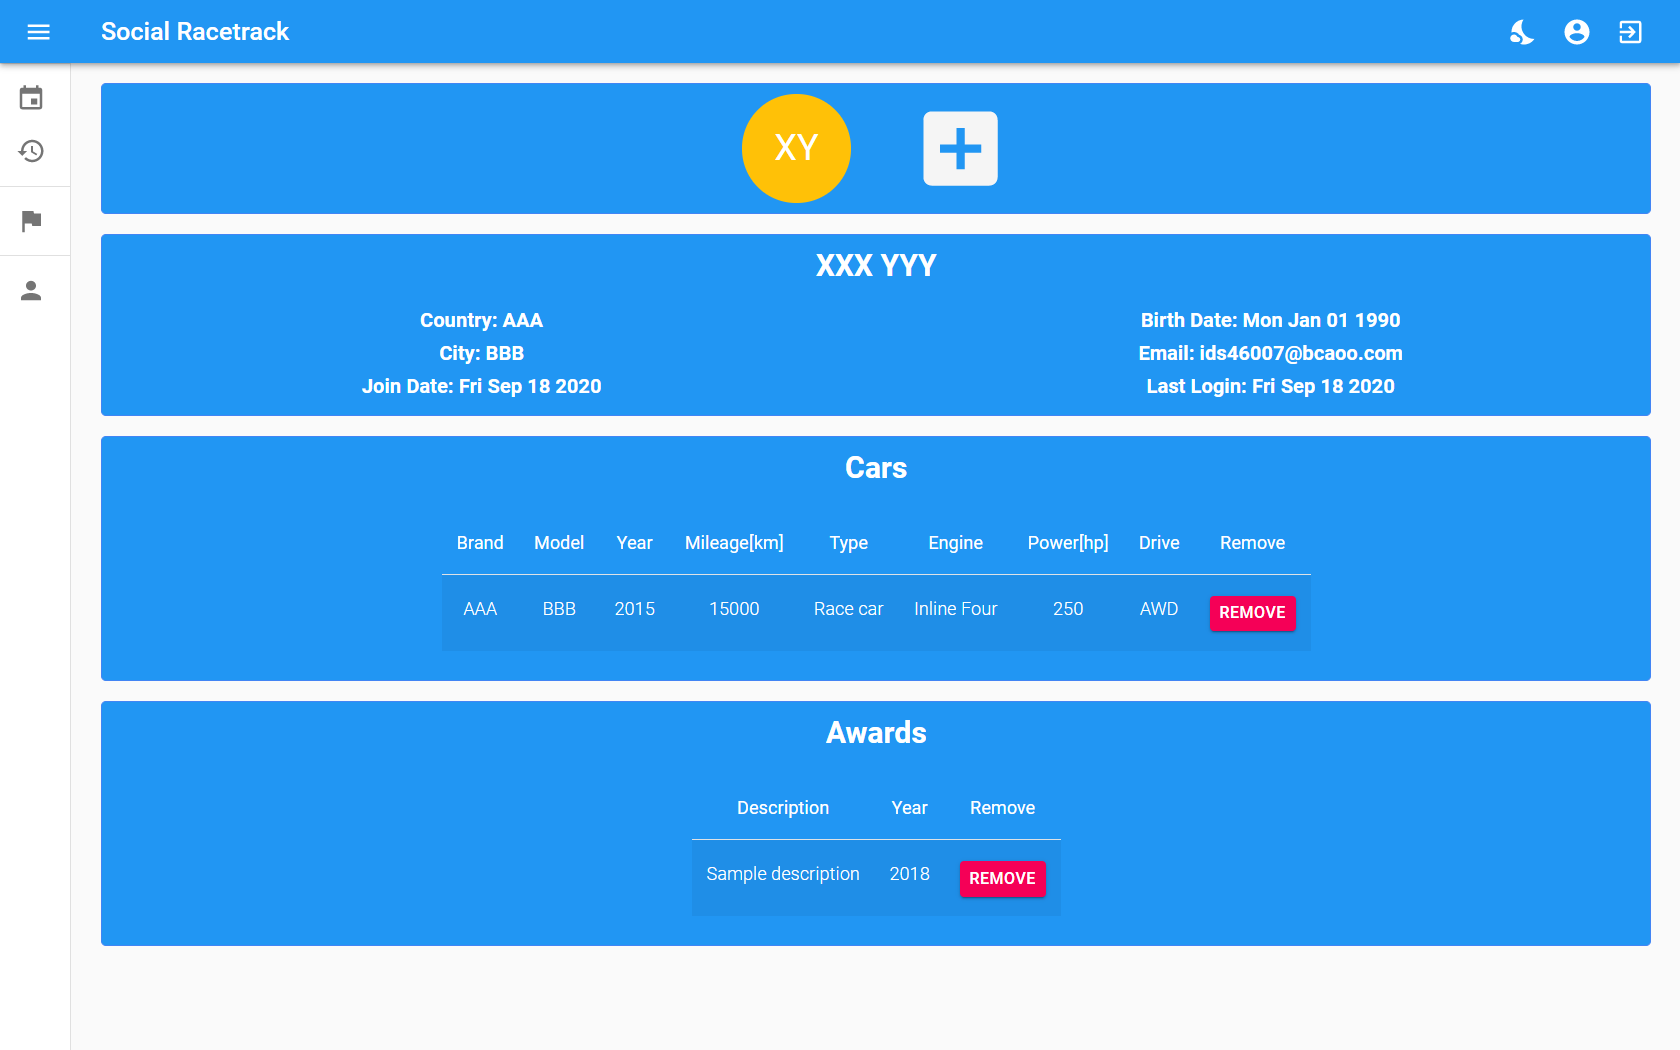
\includegraphics[width=0.7\textwidth, keepaspectratio]
                {img/chapter5/loggedin/user_panel.png}
                \caption
                [Panel konta użytkownika]
                {Panel konta użytkownika}
                \label{chapter5:dok_uzytkownika:funkc_uzyt_zalog:user_panel}
            \end{figure}

            \begin{figure}[H]
                \centering
                
\includegraphics[width=0.08\textwidth, keepaspectratio]
                {img/chapter5/loggedin/add_button.png}
                \caption
                [Przycisk dodawania i edycji panelu użytkownika]
                {Przycisk dodawania i edycji panelu użytkownika}
                \label{chapter5:dok_uzytkownika:funkc_uzyt_zalog:add_button}
            \end{figure}

            \subsubsection{Dodawanie i usuwanie floty pojazdów}
            \label{chapter5:dok_uzytkownika:funkc_uzyt_zalog:konto_uzyt:dod_usun_samochod} {
                Aby mieć możliwość dodania nowego pojazdu, należy nacisnąć przycisk
                \textit{ADD CAR} a~następnie wypełnić formularz zgodnie z~opisami jego
                pól i~zatwierdzić przyciskiem \textit{CONFIRM}. Sam formularz został
                przedstawiony na rysunku
                \ref{chapter5:dok_uzytkownika:funkc_uzyt_zalog:add_car}. W~celu
                usunięcia wybranego pojazdu należy w~panelu użytkownika przedstawionego
                na rysunku \ref{chapter5:dok_uzytkownika:funkc_uzyt_zalog:user_panel}
                nacisnąć przycisk \textit{REMOVE} przy wybranym pojeździe.

                \begin{figure}[H]
                    \centering
                    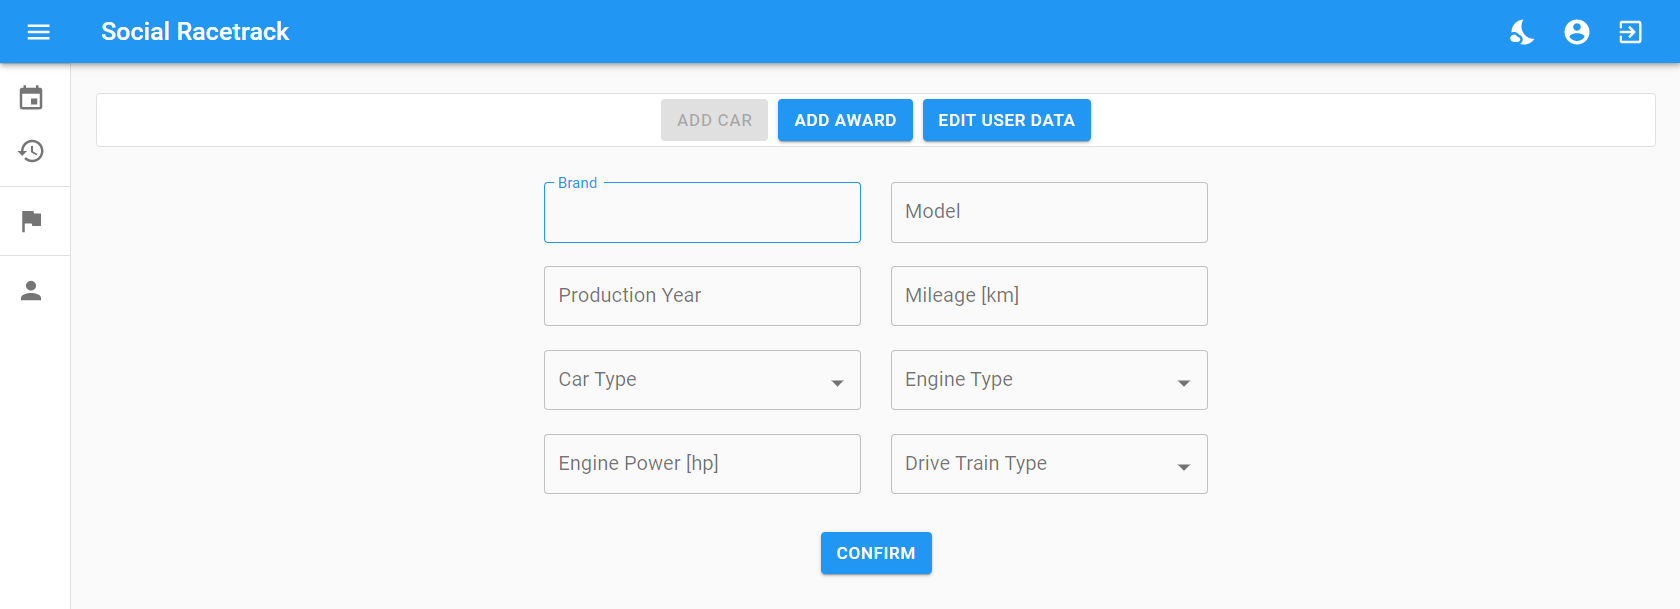
\includegraphics[width=0.8\textwidth, keepaspectratio]
                    {img/chapter5/loggedin/add_car.png}
                    \caption
                    [Panel dodawania floty pojazdów użytkownika]
                    {Panel dodawania floty pojazdów użytkownika}
                    \label{chapter5:dok_uzytkownika:funkc_uzyt_zalog:add_car}
                \end{figure}
            }

            \subsubsection{Dodawanie i usuwanie zdobytych nagród}
            \label{chapter5:dok_uzytkownika:funkc_uzyt_zalog:konto_uzyt:dod_usun_nagrody} {
                Aby mieć możliwość dodawania nowych osiągnięć, należy nacisnąć przycisk
                \textit{ADD AWARD} a~następnie wypełnić formularz zgodnie z~opisami jego
                pól i~zatwierdzić przyciskiem \textit{CONFIRM}. Sam formularz został
                przedstawiony na rysunku
                \ref{chapter5:dok_uzytkownika:funkc_uzyt_zalog:add_award}. W~celu
                usunięcia wybranego osiągnięcia sportowego należy w~panelu użytkownika
                przedstawionego na rysunku
                \ref{chapter5:dok_uzytkownika:funkc_uzyt_zalog:user_panel}
                nacisnąć przycisk \textit{REMOVE} przy wybranym osiągnięciu.

                \begin{figure}[H]
                    \centering
                    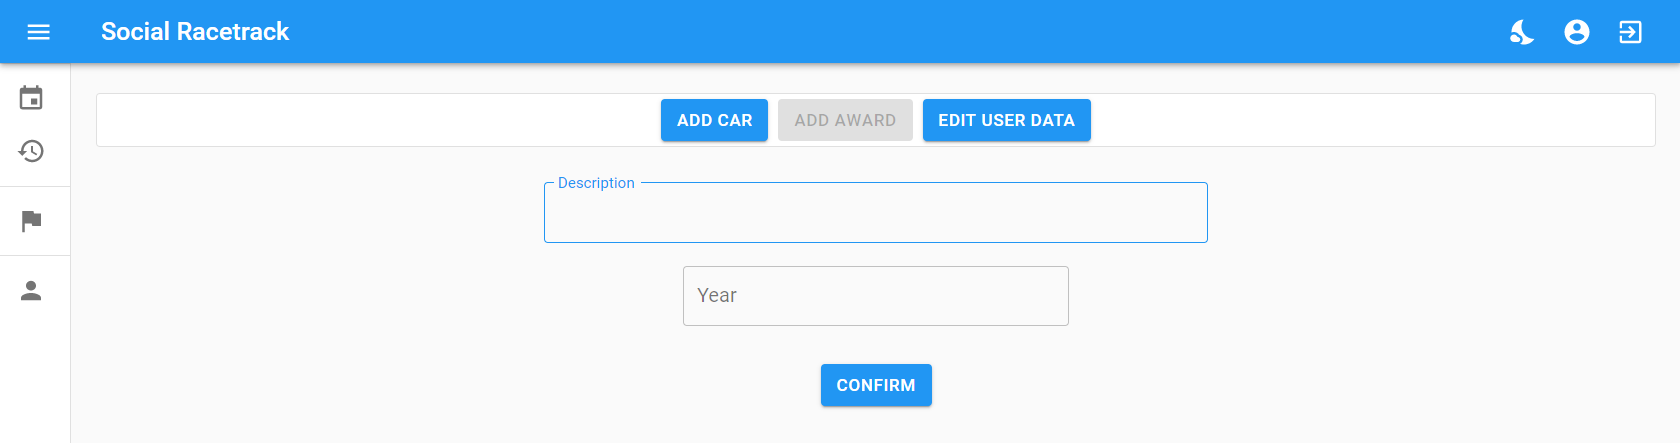
\includegraphics[width=0.8\textwidth, keepaspectratio]
                    {img/chapter5/loggedin/add_award.png}
                    \caption
                    [Panel dodawania osiągnięć sportowych użytkownika]
                    {Panel dodawania osiągnięć sportowych użytkownika}
                    \label{chapter5:dok_uzytkownika:funkc_uzyt_zalog:add_award}
                \end{figure}
            }

            \subsubsection{Edycja danych osobowych}
            \label{chapter5:dok_uzytkownika:funkc_uzyt_zalog:konto_uzyt:edycja_danych} {
                Aby dokonać edycji danych osobowych należy nacisnąć przycisk
                \textit{EDIT USER DATA} a~następnie dokonać wybranych zmian w~formularzu
                i~zatwierdzić przyciskiem \textit{CONFIRM}. Sam formularz został
                przedstawiony na rysunku
                \ref{chapter5:dok_uzytkownika:funkc_uzyt_zalog:edit_user_data}.

                \begin{figure}[H]
                    \centering
                    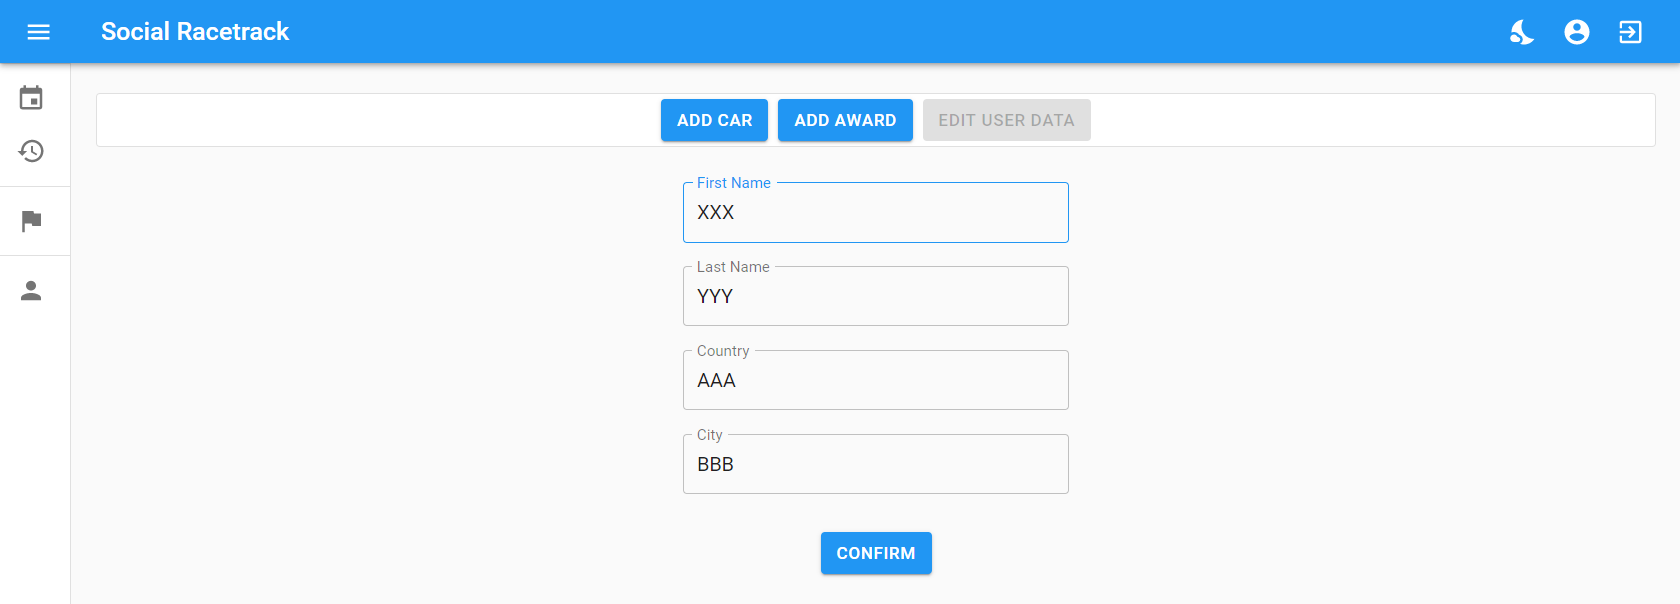
\includegraphics[width=0.8\textwidth, keepaspectratio]
                    {img/chapter5/loggedin/edit_user_data.png}
                    \caption
                    [Panel edycji danych osobowych użytkownika]
                    {Panel edycji danych osobowych użytkownika}
                    \label{chapter5:dok_uzytkownika:funkc_uzyt_zalog:edit_user_data}
                \end{figure}
            }
        }

        \subsection{Przeglądanie, dołączanie do wydarzeń i rezygnacja z udziału}
        \label{chapter5:dok_uzytkownika:funkc_uzyt_zalog:przeglad_wydarz} {
            Wydarzenia w~aplikacje są podzielone ze względu na datą, kiedy się odbyły
            lub się odbędą. Aby uzyskać dostęp do przeszłych wydarzeń należy nacisnąć
            przycisk \textit{Past Events} natomiast dla przyszłych wydarzeń należy
            nacisnąć przycisk \textit{Future Events}, obydwa przyciski znajdują się
            w~bocznym panelu a~ich użycie zostało opisane w sekcji
            \ref{chapter5:dok_uzytkownika:wprowadzenie_interface}. Wyświetlanie
            i~przeglądanie jest identyczne dla dwóch rodzajów wydarzeń, mając uruchomiony
            panel czy to przeszłych czy to przyszłych wydarzeń, są wyświetlane one
            w~formie kart. Panel ten został przedstawiony na rysunku
            \ref{chapter5:dok_uzytkownika:funkc_uzyt_zalog:przeglad_wydarz:future_events_panel}.
            Aby uzyskać więcej informacji na jego temat należy nacisnąć myszką na
            wybrane wydarzenie i~zostanie pokazany panel szczegółów wydarzenia, który
            został przedstawiony na rysunku
            \ref{chapter5:dok_uzytkownika:funkc_uzyt_zalog:przeglad_wydarz:event_details}.
            Dołączanie do wydarzenia jest możliwe poprzez naciśniecie przycisku
            \textit{PARTICIPATE IN THE EVENT} i~jest on dostępny tylko wtedy, gdy dany
            użytkownik nie bierze w nim udziału. Rezygnacja z~udziału odbywa się
            analogicznie do dołączenia czyli poprzez naciśnięcie przycisku
            \textit{CANCEL PARTICIPATION}. Jest on dostępny tylko wtedy, gdy dany
            użytkownik bierze udział w wydarzeniu.

            \begin{figure}[H]
                \centering
                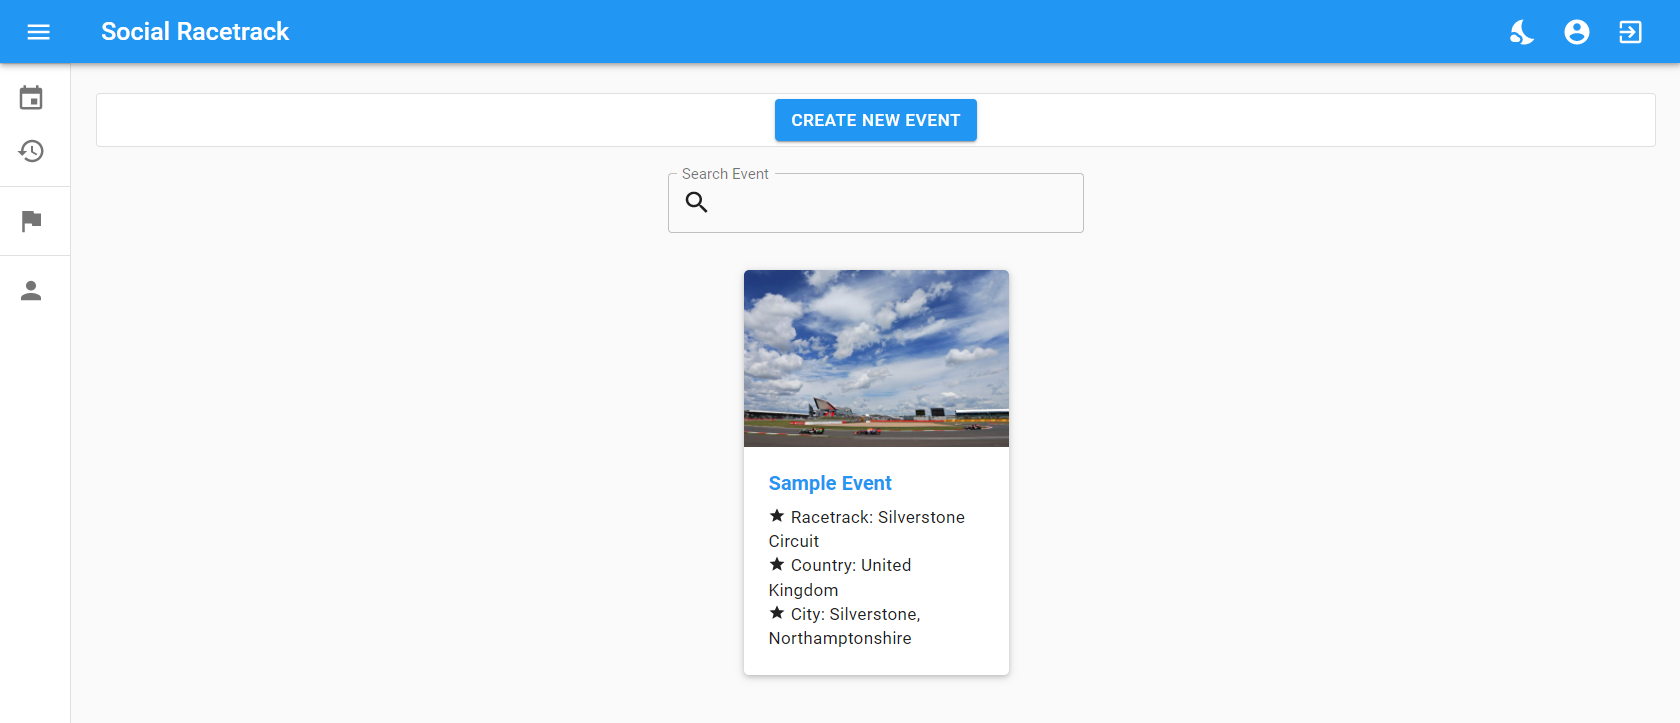
\includegraphics[width=0.8\textwidth, keepaspectratio]
                {img/chapter5/loggedin/future_event_panel.png}
                \caption
                [Panel przyszłych wydarzeń]
                {Panel przyszłych wydarzeń}
                \label{chapter5:dok_uzytkownika:funkc_uzyt_zalog:przeglad_wydarz:future_events_panel}
            \end{figure}

            \begin{figure}[H]
                \centering
                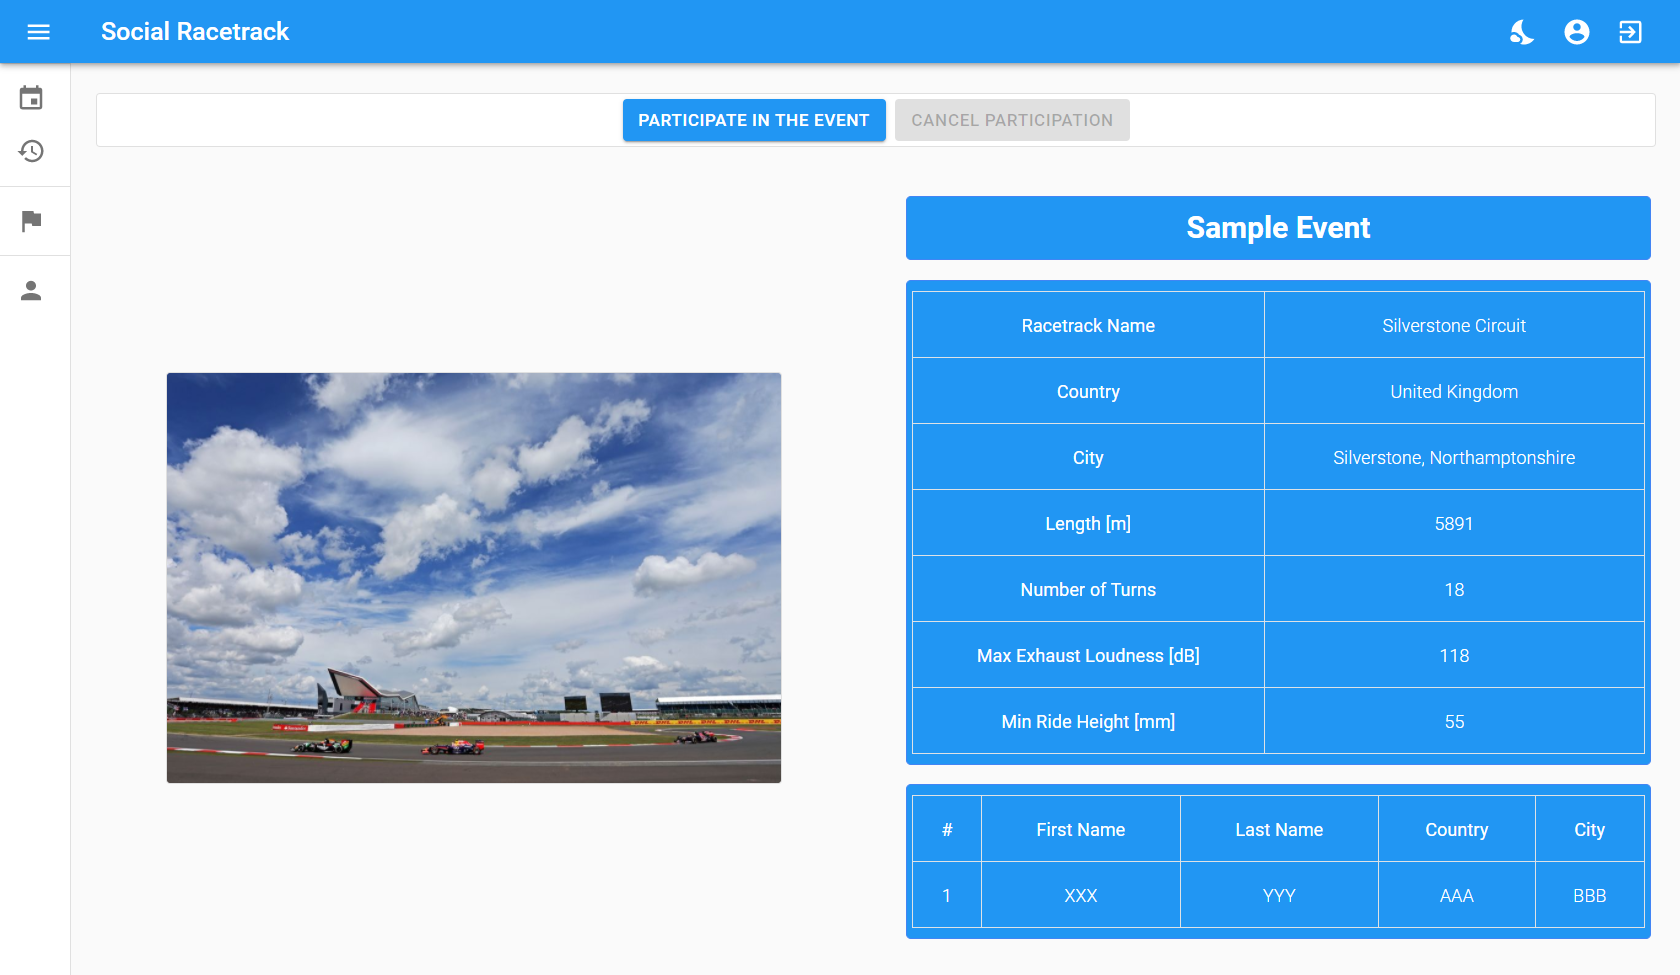
\includegraphics[width=0.8\textwidth, keepaspectratio]
                {img/chapter5/loggedin/event_details.png}
                \caption
                [Panel szczegółów wydarzenia]
                {Panel szczegółów wydarzenia}
                \label{chapter5:dok_uzytkownika:funkc_uzyt_zalog:przeglad_wydarz:event_details}
            \end{figure}
        }

        \subsection{Tworzenie wydarzeń}
        \label{chapter5:dok_uzytkownika:funkc_uzyt_zalog:tworz_wydarz} {
            W~celu stworzenia wydarzenia należy uruchomić panel przyszłych wydarzeń,
            który został pokazany na rysunku
            \ref{chapter5:dok_uzytkownika:funkc_uzyt_zalog:przeglad_wydarz:future_events_panel}.
            Następnie należy nacisnąć przycisk \textit{CREATE NEW EVENT} i~wypełnić
            formularz zgodnie z~opisem przy każdym polu oraz nacisnąć przycisk
            \textit{CONFIRM}. Formularz został przedstawiony na rysunku
            \ref{chapter5:dok_uzytkownika:funkc_uzyt_zalog:tworz_wydarz:create_event}.

            \begin{figure}[H]
                \centering
                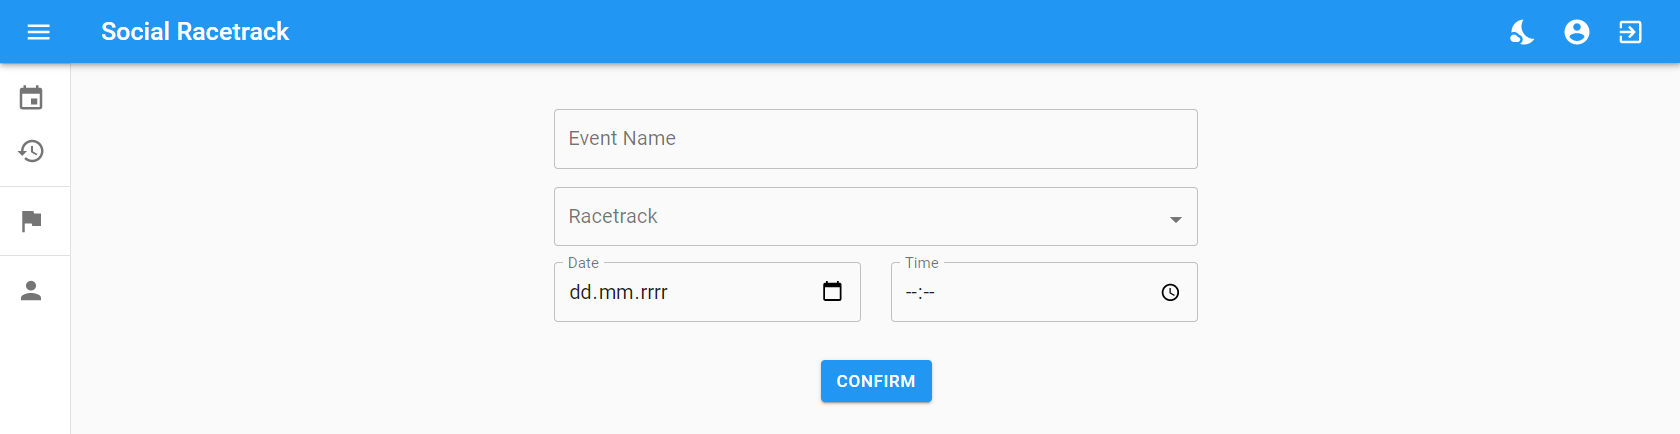
\includegraphics[width=0.8\textwidth, keepaspectratio]
                {img/chapter5/loggedin/create_event.png}
                \caption
                [Panel tworzenia wydarzeń]
                {Panel tworzenia wydarzeń}
                \label{chapter5:dok_uzytkownika:funkc_uzyt_zalog:tworz_wydarz:create_event}
            \end{figure}
        }

        \subsection{Przeglądanie kont innych użytkowników}
        \label{chapter5:dok_uzytkownika:funkc_uzyt_zalog:przeglad_kont} {
            Aby mieć możliwość przeglądania kont innych użytkowników aplikacji należy
            nacisnąć przycisk \textit{Members} znajdujący się w~bocznym panelu a~jego
            użycie zostało opisane w sekcji
            \ref{chapter5:dok_uzytkownika:wprowadzenie_interface}. Konta użytkowników
            są wyświetlane w~formie kart w~panelu użytkowników aplikacji, który został
            przedstawiony na rysunku
            \ref{chapter5:dok_uzytkownika:funkc_uzyt_zalog:przeglad_kont:members_panel}.
            Aby uzyskać więcej informacji na jego temat należy nacisnąć myszką na
            wybrane konto użytkownika i~zostanie pokazany panel szczegółów użytkownika
            aplikacji, który został przedstawiony na rysunku
            \ref{chapter5:dok_uzytkownika:funkc_uzyt_zalog:przeglad_kont:member_details}.

            \begin{figure}[H]
                \centering
                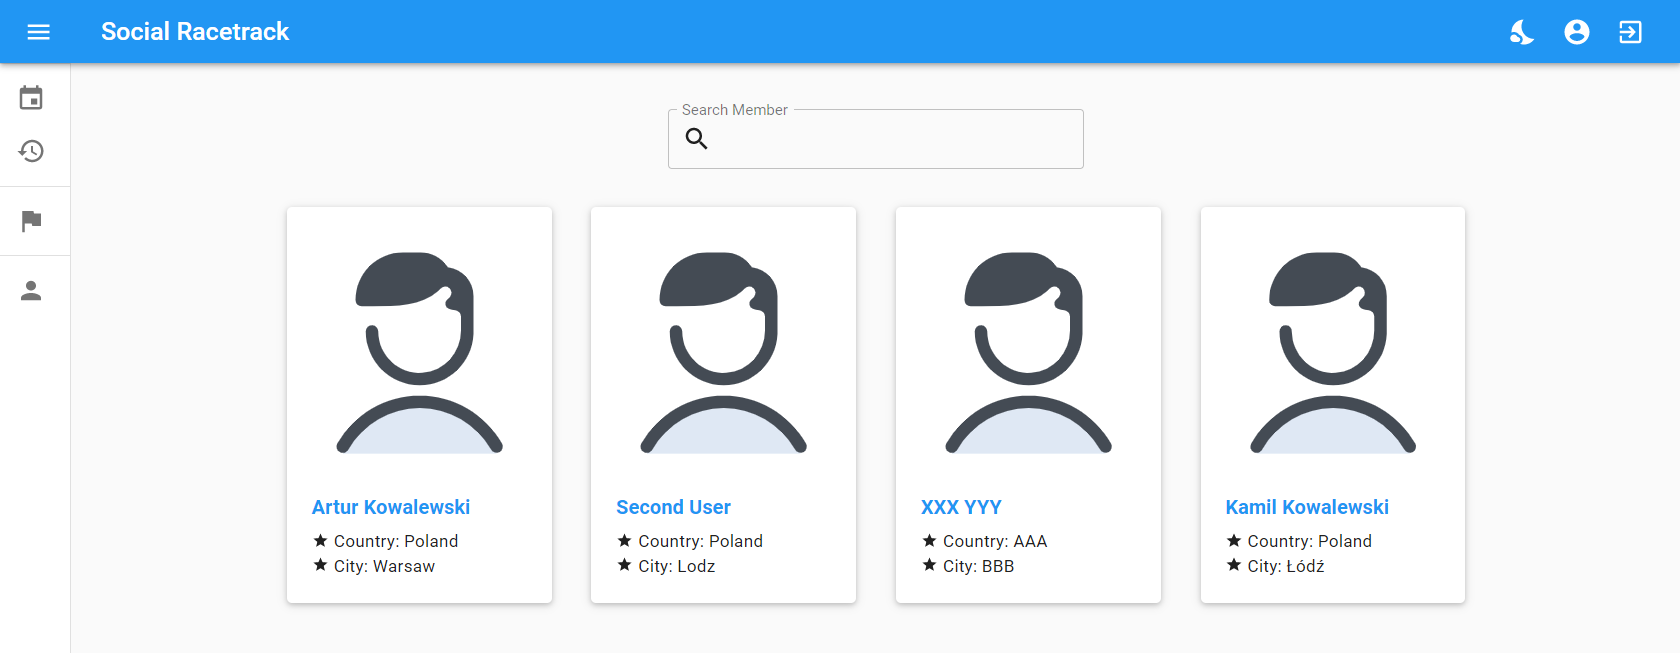
\includegraphics[width=0.8\textwidth, keepaspectratio]
                {img/chapter5/loggedin/members_panel.png}
                \caption
                [Panel użytkowników aplikacji]
                {Panel użytkowników aplikacji}
                \label{chapter5:dok_uzytkownika:funkc_uzyt_zalog:przeglad_kont:members_panel}
            \end{figure}

            \begin{figure}[H]
                \centering
                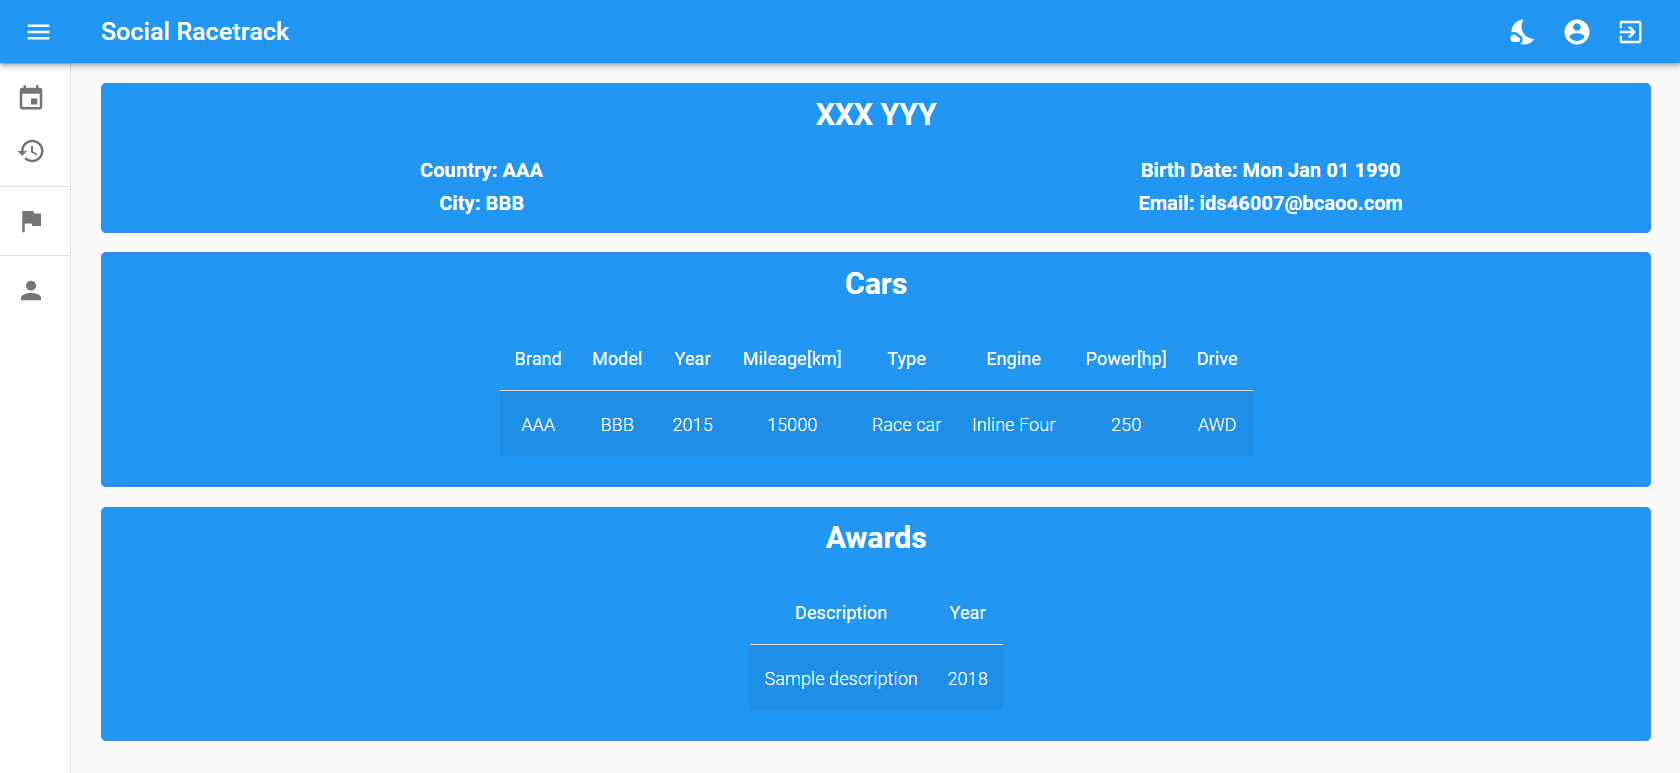
\includegraphics[width=0.8\textwidth, keepaspectratio]
                {img/chapter5/loggedin/member_details.png}
                \caption
                [Panel szczegółów innych użytkowników aplikacji]
                {Panel szczegółów innych użytkowników aplikacji}
                \label{chapter5:dok_uzytkownika:funkc_uzyt_zalog:przeglad_kont:member_details}
            \end{figure}
        }

        \subsection{Wylogowanie}
        \label{chapter5:dok_uzytkownika:funkc_uzyt_zalog:wylogowanie} {
            Aby wylogować się z~aplikacji należy nacisnąć przycisk przedstawiony na
            rysunku
            \ref{chapter5:dok_uzytkownika:funkc_uzyt_zalog:wylogowanie:logout_button},
            który znajduje się w~prawym górnym rogu.

            \begin{figure}[H]
                \centering
                
\includegraphics[width=0.1\textwidth, keepaspectratio]
                {img/chapter5/loggedin/logout_button.png}
                \caption
                [Przycisk służący do wylogowywania]
                {Przycisk służący do wylogowywania}
                \label{chapter5:dok_uzytkownika:funkc_uzyt_zalog:wylogowanie:logout_button}
            \end{figure}
        }
    }

    \section{Obsługa funkcjonalności dostępnych dla administratora}
    \label{chapter5:dok_uzytkownika:funkc_admin} {
        Aby mieć możliwości, które zostały przedstawione poniżej należy posiadać
        uprawnienia administratora. W~tym celu osoba posiadająca konto z~takimi
        uprawnieniami musi nadać osobie, która się o~nie stara aby była również
        administratorem. W~innym przypadku możliwości te nie są dostępne dla
        standardowego użytkownika. Sama informacja o~posiadaniu takich uprawnień jest
        wyświetlana w~drugiej sekcji konta użytkownika w~postaci komunikatu
        \textit{Member has admin privileges} i~jest to widoczne tylko przez
        niego oraz w~bocznym panelu w~postaci przycisku przedstawionego na rysunku
        \ref{chapter5:dok_uzytkownika:funkc_admin:admin_button}.
        Sekcje konta użytkownika zostały opisane w sekcji
        \ref{chapter5:dok_uzytkownika:funkc_uzyt_zalog:konto_uzyt}.

        \begin{figure}[H]
            \centering
            
\includegraphics[width=0.1\textwidth, keepaspectratio]
            {img/chapter5/admin/admin_button.png}
            \caption
            [Przycisk otwierający panel administratora]
            {Przycisk otwierający panel administratora}
            \label{chapter5:dok_uzytkownika:funkc_admin:admin_button}
        \end{figure}

        \subsection{Obsługa panelu administratora}
        \label{chapter5:dok_uzytkownika:funkc_admin:obsl_panel} {
            Funkcją dostępną w~tym panelu jest nadawanie uprawnień administratora. Aby
            tego dokonać należy nacisnać przycisk przedstawionego na rysunku
            \ref{chapter5:dok_uzytkownika:funkc_admin:admin_button}. Po tej akcji
            wyświetli się nowa strona z formularzem na, której należy podać adres email
            konta, które ma mieć uprawnienia administratora oraz zatwierdzić
            poprzez naciśnięcie przycisku \textit{CONFIRM}. Formularz ten został
            przedstawiony na rysunku
            \ref{chapter5:dok_uzytkownika:funkc_admin:obsl_panel:grant_admin_panel}.

            \begin{figure}[H]
                \centering
                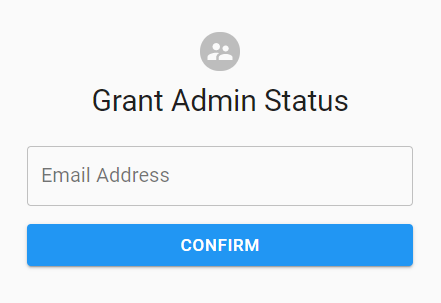
\includegraphics[width=0.4\textwidth, keepaspectratio]
                {img/chapter5/admin/grant_admin_panel.png}
                \caption
                [Panel nadawania uprawnień administratora]
                {Panel nadawania uprawnień administratora}
                \label{chapter5:dok_uzytkownika:funkc_admin:obsl_panel:grant_admin_panel}
            \end{figure}
        }

        \subsection{Usuwanie wydarzeń}
        \label{chapter5:dok_uzytkownika:funkc_admin:usun_wydarzenie} {
            Aby usunąć wydarzenie należy wyświetlić jego szczegóły przedstawione na
            rysunku
            \ref{chapter5:dok_uzytkownika:funkc_uzyt_zalog:przeglad_wydarz:event_details}
            a~następnie nacisnąć dodatkowy przycisk \textit{DELETE EVENT}, który jest
            dostępny dla administratora przedstawiony na rysunku
            \ref{chapter5:dok_uzytkownika:funkc_admin:usun_wydarzenie:remove_event_button}.
            Usuwanie wydarzeń przez administratora jest możliwe zarówno dla
            przyszłych jak i~przeszłych. Usuwanie wydarzeń, które się odbyły
            jest niezalecane.

            \begin{figure}[H]
                \centering
                
\includegraphics[width=0.8\textwidth, keepaspectratio]
                {img/chapter5/admin/remove_event_button.png}
                \caption
                [Przycisk usuwanie wydarzenia]
                {Przycisk usuwanie wydarzenia}
                \label{chapter5:dok_uzytkownika:funkc_admin:usun_wydarzenie:remove_event_button}
            \end{figure}
        }

        \subsection{Dodawanie i usuwanie torów wyścigowych}
        \label{chapter5:dok_uzytkownika:funkc_admin:dod_usun_tor} {
            W~celu dodanie nowego obiektu sportowego należy w~bocznym panelu należy
            nacisnąć przycisk \textit{Racetracks}. Po tej akcji zostanie wyświetlony
            panel przedstawiony na rysunku
            \ref{chapter5:dok_uzytkownika:obsluga_niezalogowany:racetracks}
            z~dodatkowym przyciskiem \textit{ADD NEW RACETRACK} przedstawionym na rysunku
            \ref{chapter5:dok_uzytkownika:funkc_admin:dod_usun_tor:new_racetrack_button}.
            Należy go nacisnąć a następnie zostanie wyświetlony formularz przedstawiony na
            na rysunku
            \ref{chapter5:dok_uzytkownika:funkc_admin:dod_usun_tor:add_racetrack},
            który należy wypełnić zgodnie z~opisem przy każdym polu oraz nacisnąć przycisk
            \textit{CONFIRM}.

            Aby usunąć wybrany obiekt sportowy należy wyświetlić szczegóły obiektu
            sportowego, pokazanego na rysunku
            \ref{chapter5:dok_uzytkownika:obsluga_niezalogowany:racetrack_details}
            a~następnie nacisnąć przycisk \textit{DELETE RACETRACK}, który został
            przedstawiony na rysunku
            \ref{chapter5:dok_uzytkownika:funkc_admin:dod_usun_tor:delete_racetrack}.

            \begin{figure}[H]
                \centering
                
\includegraphics[width=0.9\textwidth, keepaspectratio]
                {img/chapter5/admin/new_racetrack_button.png}
                \caption
                [Przycisk dodawania nowego obiektu sportowego]
                {Przycisk dodawania nowego obiektu sportowego}
                \label{chapter5:dok_uzytkownika:funkc_admin:dod_usun_tor:new_racetrack_button}
            \end{figure}

            \begin{figure}[H]
                \centering
                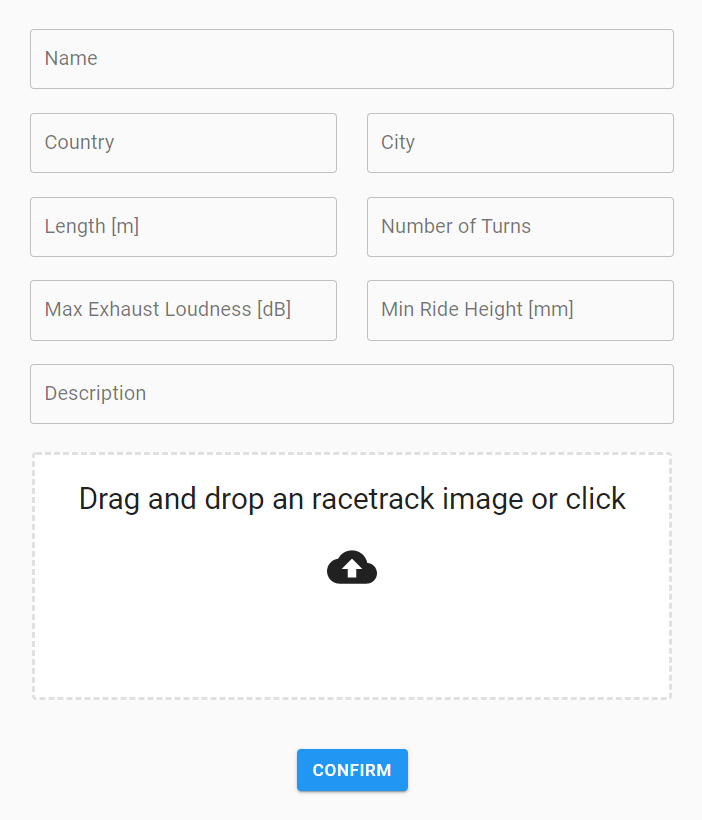
\includegraphics[width=0.4\textwidth, keepaspectratio]
                {img/chapter5/admin/add_racetrack.png}
                \caption
                [Panel dodawania nowego obiektu sportowego]
                {Panel dodawania nowego obiektu sportowego}
                \label{chapter5:dok_uzytkownika:funkc_admin:dod_usun_tor:add_racetrack}
            \end{figure}

            \begin{figure}[H]
                \centering
                
\includegraphics[width=0.8\textwidth, keepaspectratio]
                {img/chapter5/admin/delete_racetrack_button.png}
                \caption
                [Przycisk usuwania obiektu sportowego]
                {Przycisk usuwania obiektu sportowego}
                \label{chapter5:dok_uzytkownika:funkc_admin:dod_usun_tor:delete_racetrack}
            \end{figure}
        }
    }
}
\end{document}
